The microscope is a device that performs extremely important functions for human knowledge, in theoretical or empirical aspects. It is able to provide magnified views of small objects and structures. Currently, several variations of the
microscope are broadly used, which enables us to investigate much smaller spaces than those visible to the naked eye \cite{wu2008microscope}.

Microscopes are broadly used. Within biology, the areas of physiology, histology, taxonomy, cytology and molecular biology stand out; interdisciplinary knowledge areas such as materials sciences also apply microscopy, and health professionals use them in large scale for practical procedures, clinical analysis and also in research. High throughput microscopy is an important technique for the diagnosis and treatment of genetic diseases; however, to make it acceptable in the clinical environment, it is of great importance to perform high-resolution image acquisition, since low levels of sharpness can directly affect the diagnostic accuracy \cite{qiu2013evaluations}.

The advances in technologies and methods from microscopy currently show a natural trend of interdisciplinary research with image processing. This bond dates back to the middle of the 20th century, when some techniques for capturing and manipulating images, primarily developed for televisions, could be
applied to microscopy images \cite{wu2008microscope}. A classic example is noise reduction, which is an important step for cryoelectronic microscopy and also for energy filtering in transmission electron microscopy, before the 3D reconstruction process on \sigla{CT}{Computed Tomography} scans. High noise levels hinder the necessary alignment in the reconstruction task \cite{vyas2017multiscale}.

\section{Motivation}

Biological and biomedical analysis procedures performed using microscopy images also employ image processing algorithms to obtain better results. In this sense, the concept of focus is an element of great importance. The microscopically analyzed surfaces and structures are \emph{a priori} smooth and homogeneous to the naked eye; when magnified, these images show that those elements are irregular, i.e. they have different depths (when considering an upper view), textures and topologies. It is therefore necessary to constantly adjust the focus to get the image with the least amount of noise and lower frequency of blurred. Figure \ref{fig:ctenanthe} illustrates the problem of differences in depth of focus in a histological image of a \emph{Ctenanthe oppenheimiana} specimen. The focus was adjusted to the greenish central region comprised between the ribs (white band) of the leaf; so the effect of blur was kept on the ribs and their surroundings.

\begin{figure}[htb]
	\centering
	\caption{\label{fig:ctenanthe}Example of a microscopy image with sharpness problem due to focus adjustment.}
	\begin{center}
	    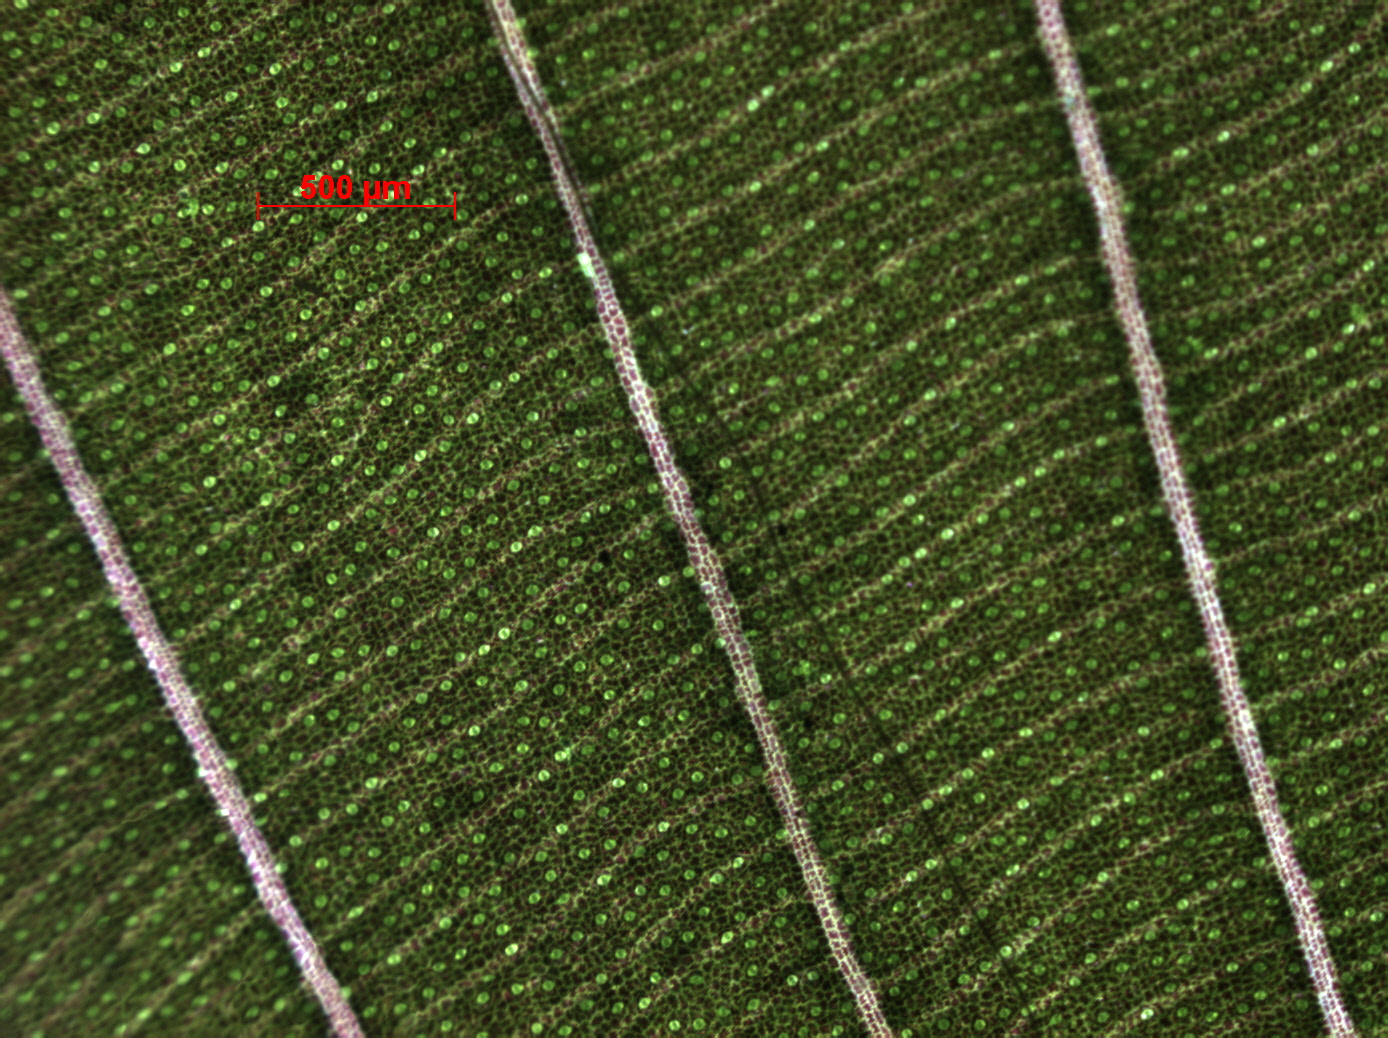
\includegraphics[scale=0.3]
			{images/fig1.png}
	\end{center}
	\centering
	\fautor
\end{figure}

There are several proposed methods to solve the sharpness problem in microscopy images, mostly based on image restoration techniques. According to \citeonline{ponti2016image}, the most frequently used iterative method in microscopic image restoration is the Richardson-Lucy algorithm. This is a particular case of the Maximum Likelihood Expectation Maximization algorithm with spectral extrapolation properties, which assists in the execution process at low conditions of \sigla{SNR}{Signal-to-Noise-Ratio}. Some examples presented by \cite{sun2005autofocusing} consist of
four classes: \emph{derivative algorithms}, \emph{statistical algorithms}, \emph{histogram-based algorithms} and \emph{intuitive algorithms}. Among these applications, derivative methods deserve more credit. The Fourier Transform proved itself to be
effective for low or moderate noise levels; in highly noisy environments, the resulting images were not satisfactory \cite{richardson1972bayesian}. From this evidence, probabilistic methods based on the Bayes Theorem were developed and provided images with better contrast, higher bandwidth and
edge enhancement for confocal fluorescence microscopy samples \cite{ponti2016image}.

The resulting images from such restoration processes have a higher degree of sharpness than the original ones when validated with metrics such as the \sigla{RMSE}{Root Mean Squared Error} and the \sigla{PSNR}{Peak Signal-to-Noise-Ratio} (both will be discussed further). However, the algorithms contain limitations when it comes to degradation as input; consequently, it produces degradation as output. An alternative to restoration is to use images from the same object, with different foci, in order to obtain an enhanced depth of field image with low degradation levels.

\section{Objectives and Hyphothesis}

The objective of this work is to develop a method which is capable of generating an extended depth of field image from a set of light microscopy images, acquired with different foci. The method will employ blur segmentation techniques and image fusion. The specific objectives are described as follows:

\begin{itemize}
    \item \emph{Evaluation of Blur Segmentation Methods}: Several approaches will be described to find the blur map, which employ different segmentation techniques. The aim is to find the approach that has the best behavior with multifocal light microscopy images. Based on current state-of-the-art literature, empirical results of efficiency and efficacy of the methods will be pursued, and a specific method for light microscopy will be developed. The performance evaluation relates to execution time, asymptotic complexity and blur map accuracy;
    
    
\end{itemize}

It is hypothesized that methods based on the Fourier and Wavelet Transforms may be employed to produce a reliable blur segmentation, in order to perform the multifocus image fusion and obtain an extended depth of field image.

\section{Structure of the document}

This monograph is organized as follows:

\begin{itemize}
    \item Chapter \ref{chapter:fundamentals-of-optics-and-light-microscopy} provides several essential concepts of Optics for understanding the Light Microscopy basics and the nature of blur;
    
    \item Chapter \ref{chapter:image-processing} contains the theoretical background in image processing, necessary for the comprehension of the related work and the proposed methods;
    
    \item Chapter \ref{chapter:related-work} apply the image processing basis and some other concepts with the most related relevant work in blur segmentation and multifocus image fusion areas;
    
    \item Chapter
    \ref{chapter:materials-and-methods} exposes details of the proposed approaches for solving the problem;
    
    \item Chapter \ref{chapter:preliminary-results}
    show some experimental results with artificially blurred images and real microscopy multifocus images;
    
    \item Chapter \ref{chapter:conclusions} is designed in this period for presenting the schedule of what should be done next in order to achieve the objective and use this work to contribute to science.
    
\end{itemize}
